\section{Markov Chains}

For this course, we will always take \(I\) to be a countable set and all our random variables will be defined on the same probability space \(\pqty{\Omega, \eventSpace, \Prob}\).

\begin{definition}[Markov Chain, Time-Homoegneous, Transition Matrix]
    A \term{Markov chain} is a \term{random process} (or a \term{stochastic process})
    \[
        X = \pqty{X_0, X_1, \ldots} = \pqty{X_n}_{n \geq 0}
    \]
    taking values in a discrete state space \(I\), with the property that
    \[
        \Prob\pqty{\Conditional{X_{n + 1} = x_{n + 1}}{X_n = x_n, X_{n - 1} = x_{n - 1}, \ldots, X_0 = x_0}} = \Prob\pqty{\Conditional{X_{n + 1} = x_{n + 1}}{X_n = x_n}}
    \]
    for any sequence of states \(x_0, x_1, \ldots, x_{n + 1} \in I\) and any \(n \geq 0\).

    If the probabilities \(\Prob\pqty{\Conditional{X_{n + 1} = y}{X_n = x}}\) is independent of \(n\), then the Markov chain is said to be \term{homogeneous} (or \term{time-homogeneous}). In this case, we define the \term{transition matrix}
    \[
        P = \pqty{P_{xy}}_{x, y \in I}, \quad P_{xy} = P\pqty{x, y} = \Prob\pqty{\Conditional{X_{n + 1} = y}{X_n = x}}.
    \]

    We say \(P\) is a \term{stochastic matrix} because each row is a distribution in \(I\): \(P_{xy} \geq 0\) for all \(x, y \in I\), and
    \[
        \sum_{y \in I} P_{xy} = 1, \quad \forall x \in I.
    \]
\end{definition}

\begin{figure}[ht!]
    \centering
    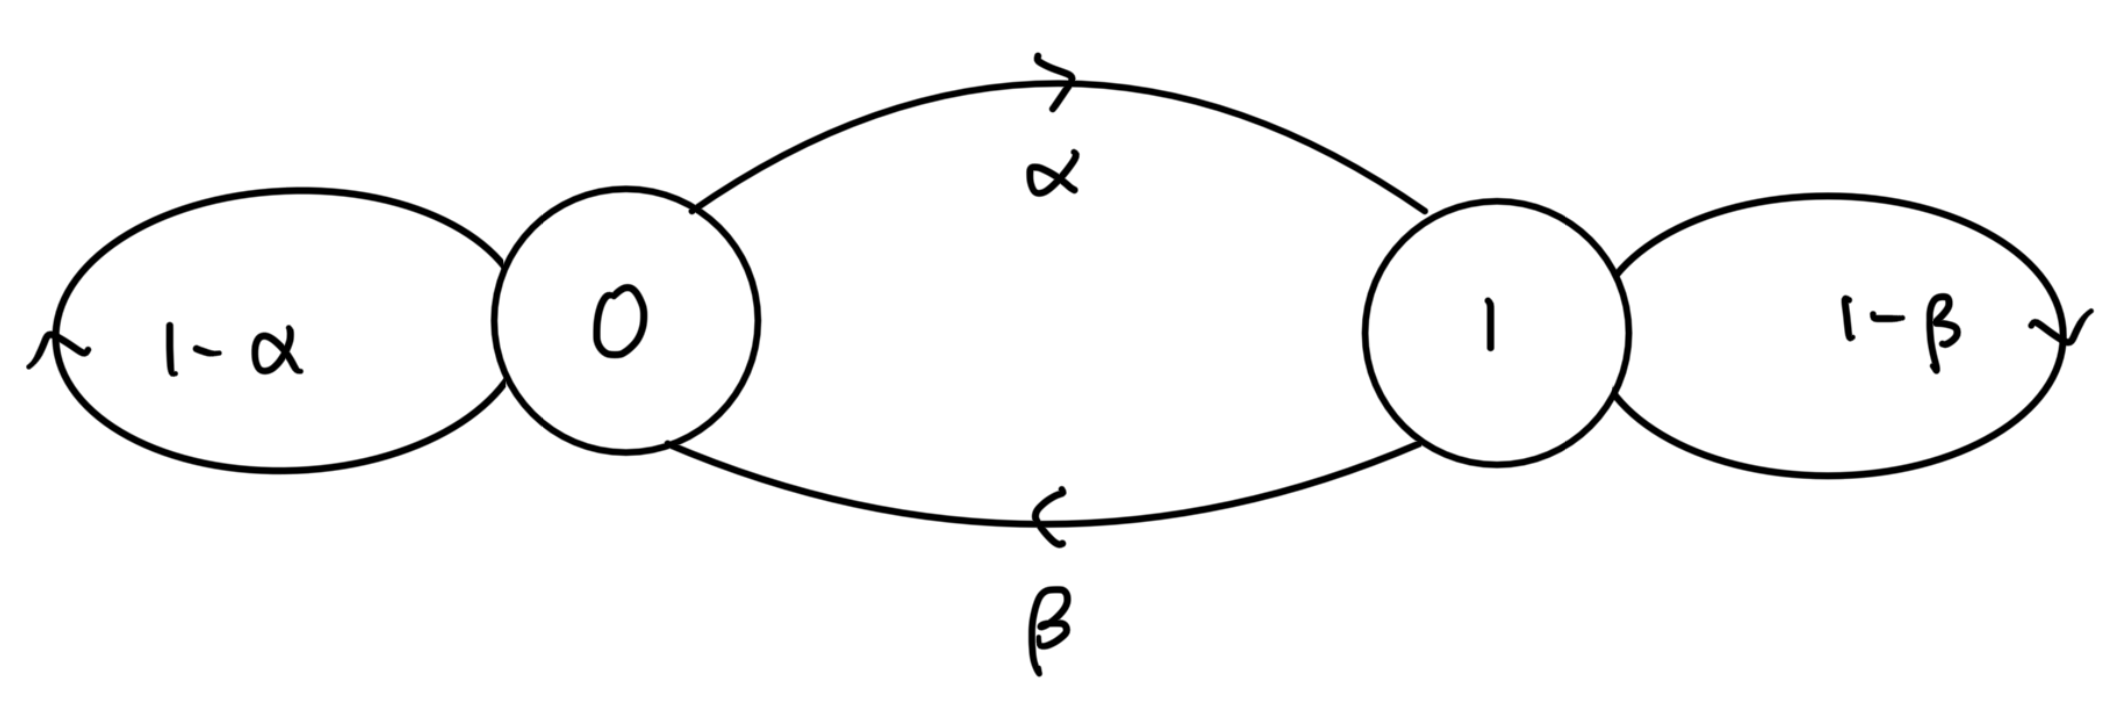
\includegraphics[width=0.75\textwidth]{fig/markov-chain-example-1.png}
    \caption{A Binary Markov chain}
\end{figure}

\begin{figure}[ht!]
    \centering
    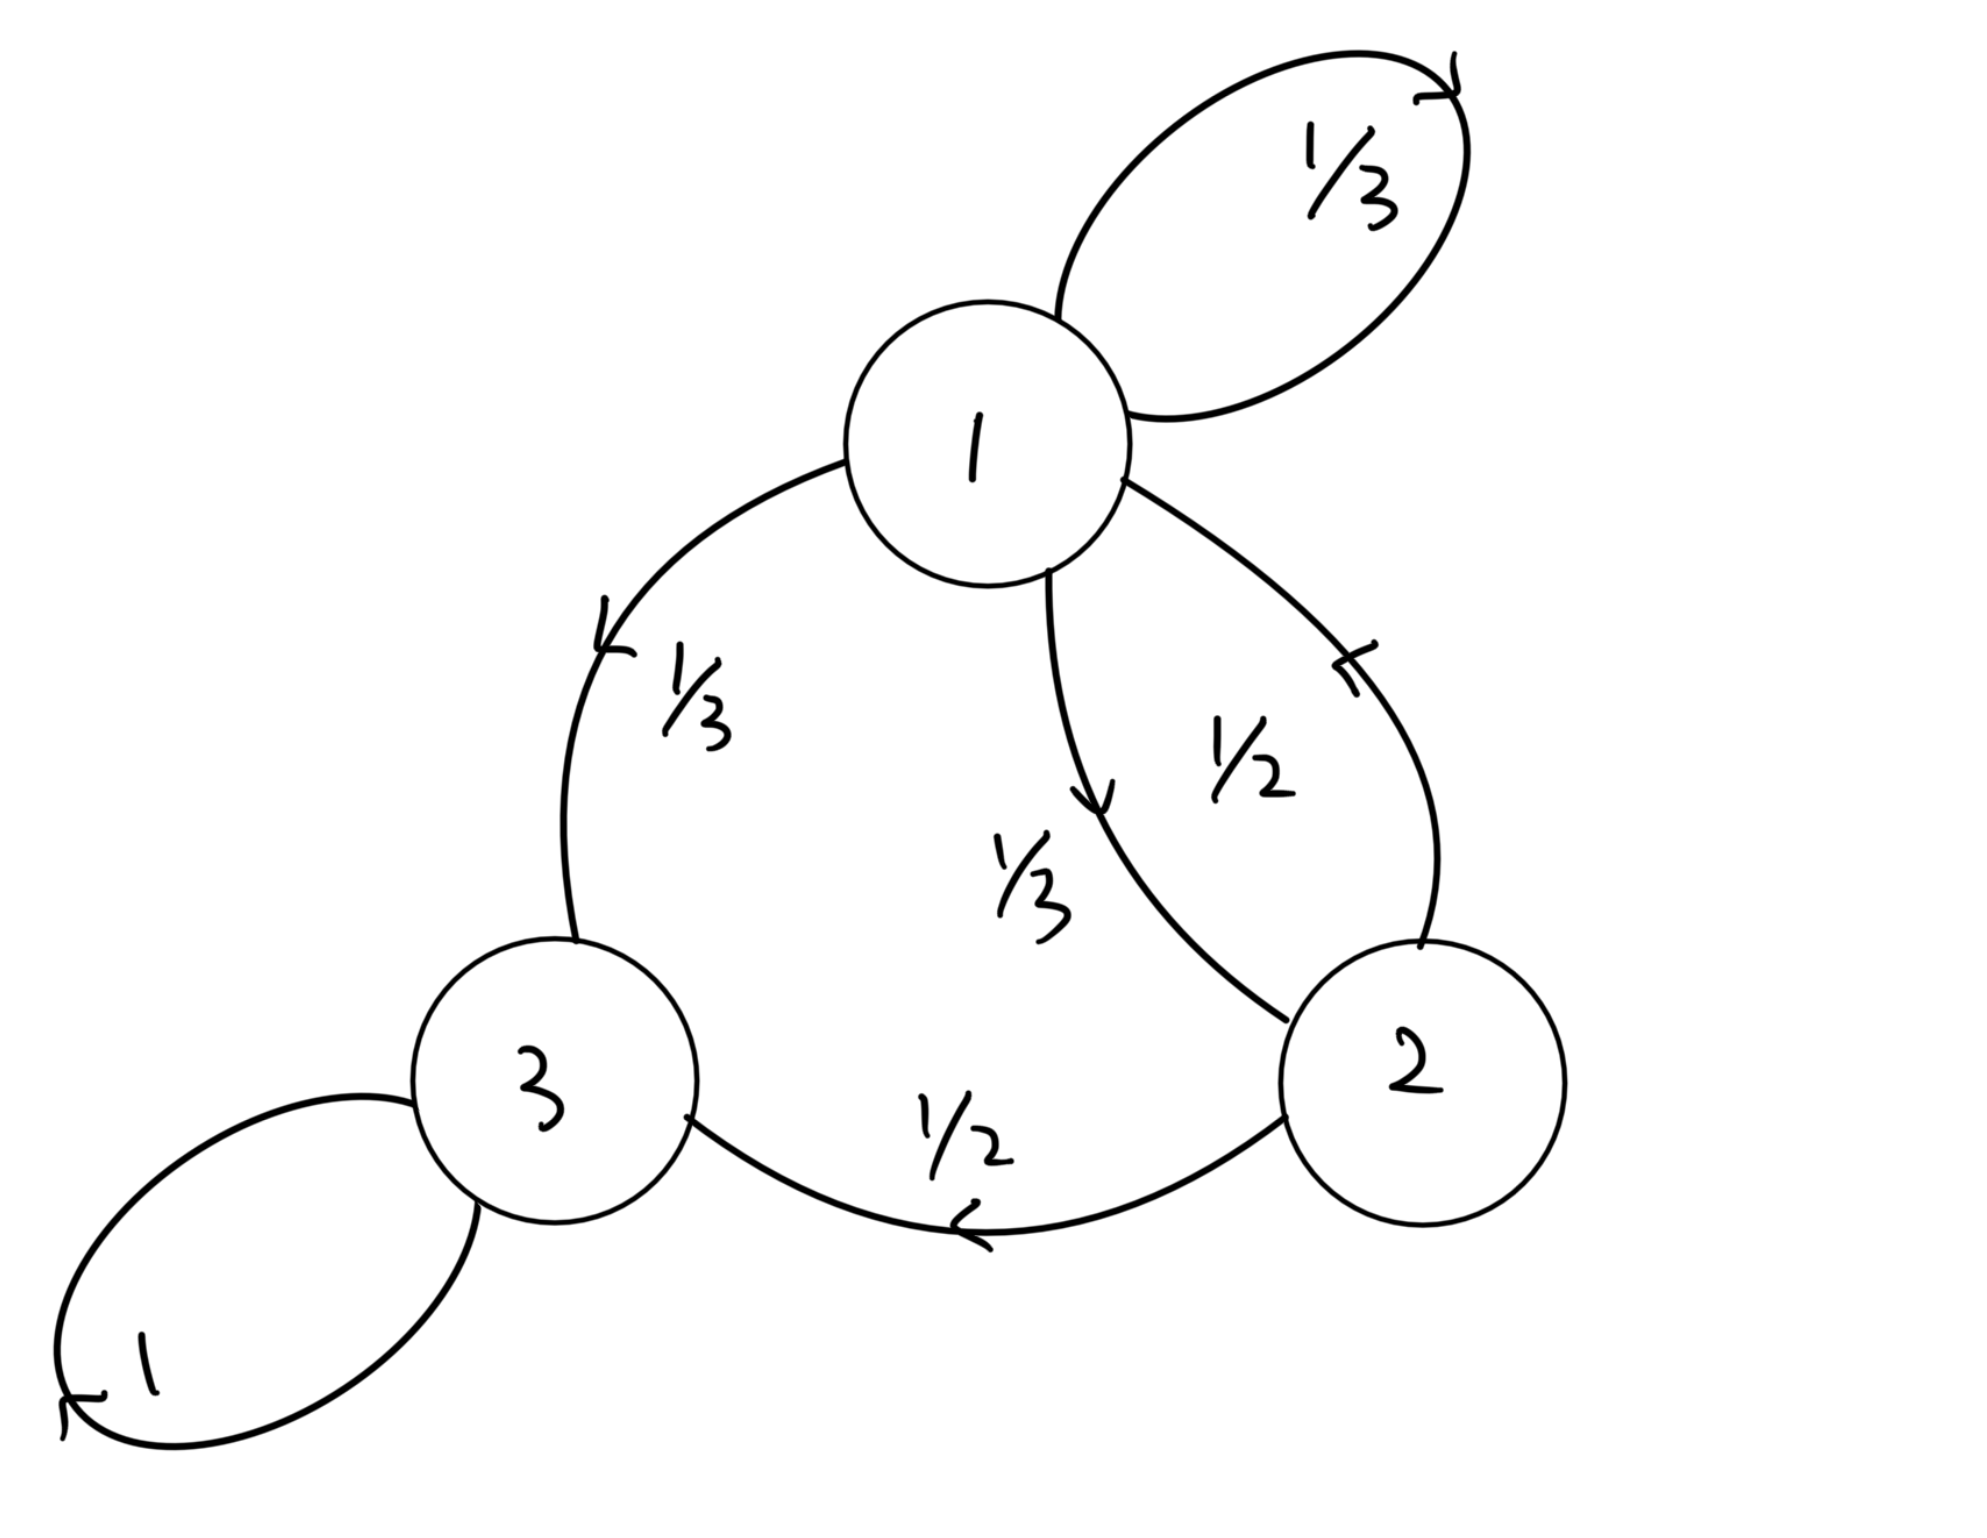
\includegraphics[width=0.75\textwidth]{fig/markov-chain-example-2.png}
    \caption{A Ternary Markov chain}
\end{figure}

\begin{examples}
    \begin{itemize}
        \item Consider the binary state \(I = \Bqty{0, 1}\), with the transition matrix
        \[
            P = \pmqty{1 - \alpha & \alpha \\ \beta & 1 - \beta}.
        \]

        \item Consider the ternary state \(I = \pqty{1, 2, 3}\), with the transition matrix
        \[
            P = \pmqty{\flatfrac{1}{3} & \flatfrac{1}{3} & \flatfrac{1}{3} \\ \flatfrac{1}{2} & 0 & \flatfrac{1}{2} \\ 0 & 0 & 1}.
        \]

        At large times, it seems like the case that the chain is in state \(3\) is absorbing, and the chain will eventually end up in state \(3\) with probability \(1\).
    \end{itemize}
\end{examples}

\begin{definition}[\(\Markov\pqty{\lambda, P}\)]
    We say a stochastic process \(X = \pqty{X_n}_{n \geq 0}\) with values in a discrete set \(I\) is \(X \sim \Markov\pqty{\lambda, P}\), where \(\lambda = \pqty{\lambda_i}_{i \in I}\) is a probability distribution on \(I\), and \(P\) is a stochastic matrix, if \(X\) is a Markov chain with transition matrix \(P\) and initial distribution \(\lambda\):
    \[
        \Prob\pqty{X_0 = i} = \lambda_i, \quad \forall i \in I.
    \]
\end{definition}

\begin{theorem}
    \(X \sim \Markov\pqty{\lambda, P}\) if and only if
    \[
        \Prob\pqty{X_0 = i_0, X_1 = i_1, \ldots, X_n = i_n} = \lambda_{i_0} P\pqty{i_0, i_1} P\pqty{i_1, i_2} \cdots P\pqty{i_{n - 1}, i_n}
    \]
    for all paths \(n \geq 0\) and \(i_0, i_1, \ldots, i_n \in I\).
\end{theorem}